\documentclass[twocolumn,a4paper,11pt]{scrartcl}

% Language and font encoding
\usepackage[spanish,es-noshorthands]{babel}
\usepackage[utf8]{inputenc}
\usepackage[T1]{fontenc}

% Other necessary packages
\usepackage{graphicx}
\usepackage{amsmath}
\usepackage{cite}
\usepackage{url}
\usepackage{hyperref}

% Additional formatting for two-column layout with centered abstract
\addto{\captionsspanish}{\renewcommand{\abstractname}{}} % quitar título del resumen

% Title information
\title{El experimento de Rutherford}
\author{Nombre del Autor}
\date{}

\begin{document}

\twocolumn[
  \begin{@twocolumnfalse}
    \maketitle
    \begin{abstract}
    \begin{center}
    \begin{minipage}{0.6\textwidth}
Describe de manera concisa el trabajo realizado en la práctica, indicando qué se hizo, cómo se hizo y a qué resultados se llegó.
\end{minipage}
\end{center}
\end{abstract}
\end{@twocolumnfalse}
]

\section{Objetivos}
En este experimento examinamos la validez del modelo atómico de Rutherford utilizando datos obtenidos a través de una simulación del experimento de dispersión de Rutherford. Mediante el análisis de estos datos simulados, buscamos corroborar las predicciones teóricas del modelo y evaluar su precisión en la descripción del comportamiento de las partículas alfa al interactuar con los núcleos atómicos. Adicionalmente, nos proponemos utilizar estos mismos datos simulados para estimar una cota superior del radio del núcleo atómico del oro. Esta estimación nos permitirá obtener una aproximación de las dimensiones nucleares, proporcionando así una valiosa información sobre la estructura atómica a escala subatómica. A través de estos objetivos, esperamos profundizar nuestra comprensión de los principios fundamentales de la física nuclear y la validez de los modelos teóricos en la descripción de fenómenos atómicos.

\section{Marco teórico}
El modelo atómico propuesto por Ernest Rutherford revolucionó nuestra comprensión de la estructura atómica. En su innovadora teoría, Rutherford postuló que toda la carga positiva de un átomo se concentra en un núcleo extremadamente pequeño y denso. Este núcleo, a pesar de su diminuto tamaño, es responsable de la dispersión de las partículas alfa cuando estas se aproximan lo suficiente como para experimentar la repulsión de la fuerza de Coulomb.

La trayectoria de una partícula alfa al ser dispersada por un núcleo atómico se puede visualizar como una curva hiperbólica. Inicialmente, la partícula se desplaza en una línea recta a una distancia 'b' de una trayectoria paralela que atraviesa el centro del núcleo. A medida que se acerca al núcleo, la partícula alfa alcanza un punto de máxima aproximación, a una distancia mínima 'r', antes de ser desviada. Esta desviación resulta en un cambio de dirección, formando un ángulo Θ con respecto a su trayectoria original.

Basándose en estas observaciones, Rutherford desarrolló un modelo matemático para describir este fenómeno. En su análisis, consideró varios factores cruciales: la carga eléctrica del núcleo atómico, la trayectoria hiperbólica de las partículas alfa, y el principio de que la cantidad de partículas dispersadas a un ángulo Θ debe ser proporcional a la cantidad de partículas en el haz incidente. Integrando estos elementos, Rutherford logró deducir una expresión que predice la distribución angular de las partículas alfa dispersadas, sentando así las bases para una comprensión cuantitativa de la estructura atómica a nivel subatómico.

\section{Diseño experimental}
El diseño experimental de esta práctica se basa en una simulación sofisticada \cite{Simulador} del experimento de dispersión de Rutherford \cite{Melissinos1968}. En este montaje virtual, se simula el lanzamiento de un haz de $10^8$ partículas alfa hacia una lámina extremadamente delgada de oro. El haz, con un área transversal de $1 mm^2$, está compuesto por partículas cuyas trayectorias son perfectamente paralelas, aunque sus posiciones dentro del haz se distribuyen aleatoriamente. Estas partículas alfa, cada una con una energía cinética de 5.5 MeV, inciden perpendicularmente sobre una lámina de oro de apenas $10^{-6}$ m de espesor.

La simulación considera meticulosamente las interacciones de cada partícula alfa con el material de la lámina de oro, determinando así la trayectoria resultante tras el impacto. Para cuantificar estas interacciones, se implementa un detector virtual capaz de contar el paso de las partículas alfa. Este detector, con un área efectiva de 4 cm², está diseñado para determinar cuántas de las partículas incidentes son dispersadas a un ángulo Θ respecto a la trayectoria original del haz.

\begin{figure}[h!]
    \centering
    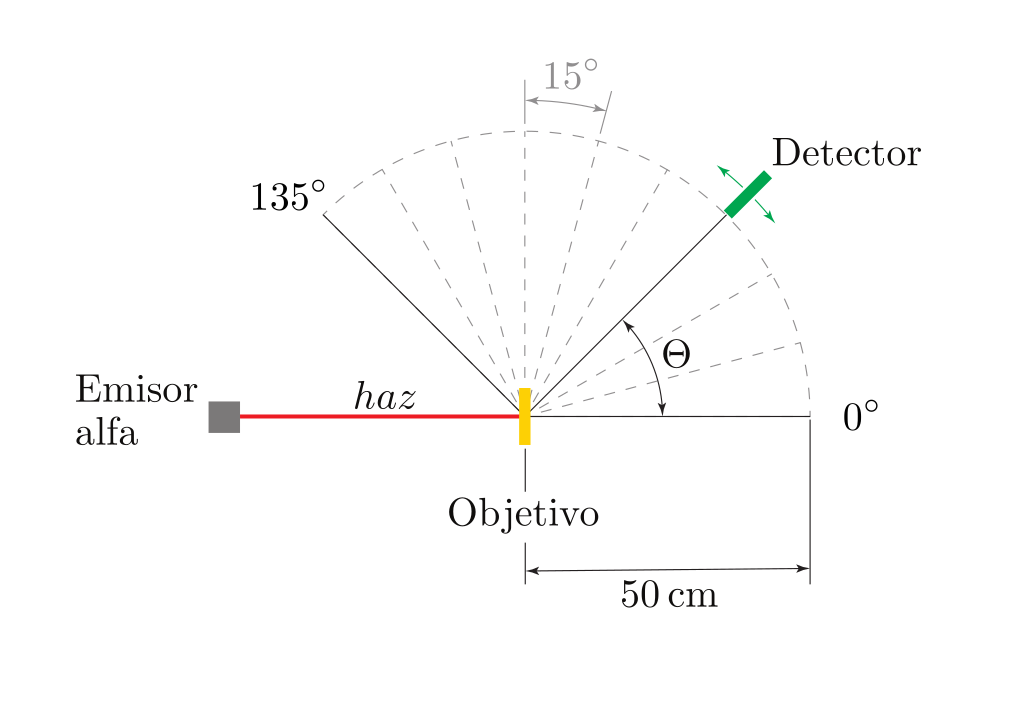
\includegraphics[width=0.4\textwidth]{simulador.png}
    \caption{Simulador del experimento de Rutherford.}
    \label{fig:simulador}
\end{figure}

Una característica clave de este montaje experimental es la movilidad del detector, como puede apreciarse en la figura \ref{fig:simulador} este puede desplazarse sobre una trayectoria circular cuyo centro coincide con el punto de impacto del haz sobre la lámina de oro. La flexibilidad del sistema permite posicionar el detector en intervalos de 15° a lo largo de un arco que abarca desde 0° hasta 135° con respecto a la dirección original del haz. Esta configuración permite una medición precisa de la distribución angular de las partículas dispersadas.

Para llevar a cabo el experimento se realizan múltiples mediciones para cada posición angular del detector, abarcando todo el rango de ángulos disponibles en el montaje experimental. Estas mediciones repetidas permiten estimar un valor medio robusto y cuantificar la incertidumbre asociada a cada punto de datos, garantizando así la fiabilidad de los resultados obtenidos.

Una vez recopilados los datos, se procede a su representación gráfica, empleando una escala logarítmica para el conteo de partículas en el detector. Luego se realiza un ajuste de los mismos a una función de la forma $I = k \sin^n (\Theta/2)$, donde $I$ representa la intensidad de partículas dispersadas, $\Theta$ el ángulo de dispersión, y $k$ y $n$ son parámetros a determinar. 

Finalmente, se procede a estimar una cota superior para el radio del núcleo atómico basándonos en el hecho de que en la distancia mínima de aproximación la energía cinética de las partículas alpha está en equilibrio con la fuerza de Coulomb repeliéndolas. De la geometría de la dispersión y de la energía de las partículas alpha incidentes se puede obtener las siguientes ecuaciones  \cite{Symon1960}:

\begin{equation}
  \begin{aligned}
    b &= \frac{Z_1Z_2}{4\pi \epsilon_0} \frac{1}{2E} \sqrt{\frac{1 + cos\theta}{1-cos\theta}} \\
    r &= \frac{b cos(\theta /2)}{1-sen(\theta /2)}
  \end{aligned}
  \label{eq:radio_nuclear}
\end{equation}

\section{Resultados y discusión}

Se realizaron cinco mediciones para cada ángulo posible del simulador, los datos en bruto se encuentran en el repositorio del laboratorio \cite{BrianDL_laboratorio} en el archivo experimento\_de\_rutherford/raw\_data.csv. 
Para cada valor del ángulo ($\theta$) tomamos el promedio de las cinco simulaciones (N) y la desviación estándard ($\sigma$) como la incertidumbre de la medición. Los resultados se muestran en la tabla \ref{tab:data1} y el en archivo data.csv del mismo repositorio y carpeta.

\begin{table}[h]
  \centering
  \begin{tabular}{cccc}
  \hline
  $\theta$ & N & $\sigma$ \\
  \hline
  0 & 28198524 & 6323 \\
  15 & 5293 & 129 \\
  30 & 295 & 14 \\
  45 & 55 & 7 \\
  60 & 23 & 3 \\
  75 & 10 & 4 \\
  90 & 3 & 2 \\
  105 & 2 & 2 \\
  120 & 2 & 2 \\
  135 & 2 & 1 \\
  \hline
  \end{tabular}
  \caption{Conteo de partículas por ángulo de incidencia}
  \label{tab:data1}
  \end{table}

La Figura \ref{fig:rutherford_dispersion} muestra la representación gráfica de estos datos, utilizando una escala logarítmica para el número de partículas detectadas.

\begin{figure}[h]
\centering
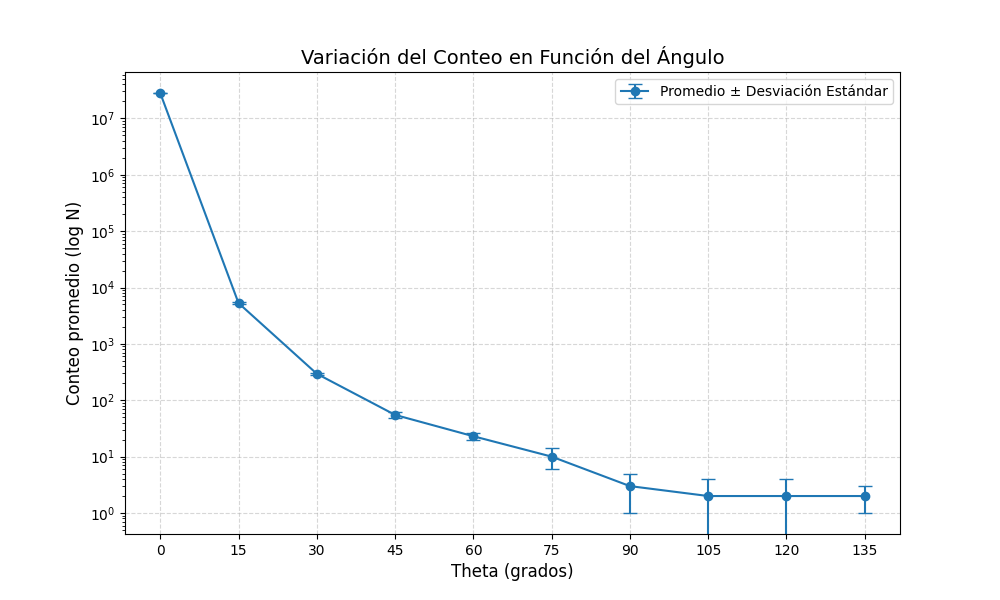
\includegraphics[width=0.4\textwidth]{data.png}
\caption{Dispersión de Rutherford: Número de partículas detectadas en función del ángulo de dispersión.}
\label{fig:rutherford_dispersion}
\end{figure}

El gráfico revela varios aspectos importantes del experimento de Rutherford:

1. La mayoría de las partículas pasan a través de la lámina de oro sin ser desviadas significativamente, como se evidencia por el alto conteo a 0°. la gran mayoría de las partículas alfa atraviesan la lámina de oro sin sufrir desviaciones significativas. Esto sugiere que el átomo es en gran parte "vacío", con la mayor parte de su volumen permitiendo el paso libre de las partículas alfa.

2. Se observa una disminución drástica en el número de partículas detectadas a medida que aumenta el ángulo de dispersión, lo cual es consistente con el modelo de Rutherford de un núcleo pequeño y denso. Y en contra del modelo atómico de Thomson que predeciría muchas partículas dispersas, ya que la mayoría de partículas alpha colisionarían con el núcleo grande y homogéneo.

3. La presencia de partículas dispersadas en ángulos grandes (incluso a 135°) contradice el modelo atómico de Thomson, que predecía solo pequeñas desviaciones.

Para cuantificar más precisamente la relación entre el ángulo de dispersión y el número de partículas detectadas, procedemos a realizar un ajuste de los datos a la función $N = k \sin^n (\theta/2)$, donde $k$ y $n$ son parámetros a determinar.

Utilizando el script de Python llamado graficar\_fit.py en el repositorio del proyecto, se ajustaron los datos experimentales a la función propuesta. Los resultados del ajuste se muestran en la Figura \ref{fig:rutherford_fit}.

\begin{figure}[h]
\centering
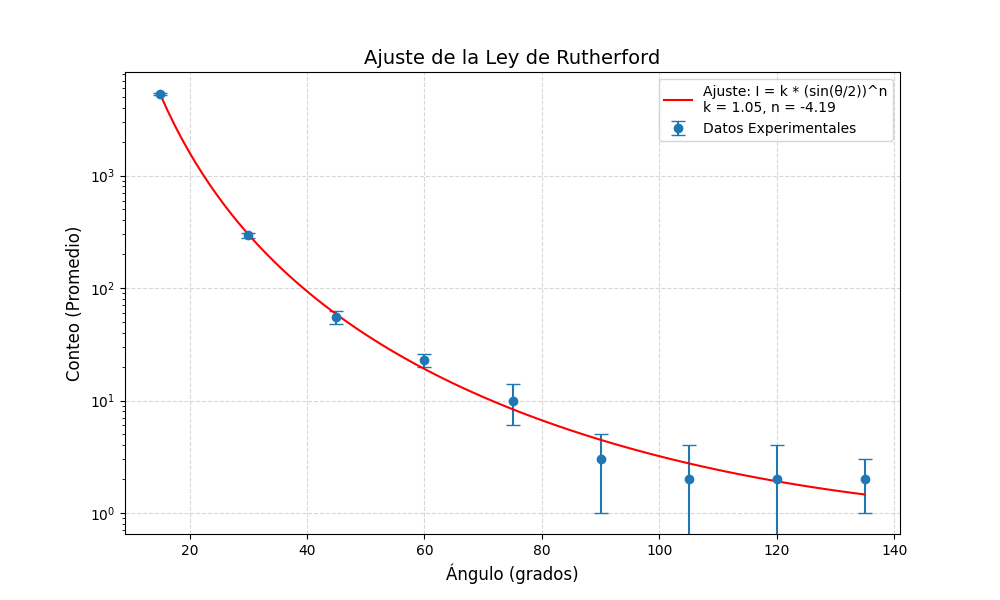
\includegraphics[width=0.4\textwidth]{data_fit.png}
\caption{Dispersión de Rutherford: Datos experimentales y curva de ajuste.}
\label{fig:rutherford_fit}
\end{figure}

El ajuste proporcionó los siguientes valores para los parámetros:

\begin{itemize}
    \item $k = 1.05 \pm 0.11$
    \item $n = 4.19 \pm 0.06$
\end{itemize}

\subsection*{Calculo del radio máximo del átomo}
Aplicando la ecuación \ref{eq:radio_nuclear} y utilizando el valor de $theta=135$ obtenido de la simulación, podemos calcular el radio máximo del átomo de oro.
Tomando los valores en SI:
\begin{itemize}
  \item $E=8.81E-13$
  \item $e=1.60E-19$
  \item $Z_1=2$
  \item $Z_2=79$
  \item $\epsilon_0=8.85E-12$
  \item $\theta = 134$
\end{itemize}

El valor obtenido para $r_{max}$ es 8.31E-14 m lo cual podemos contrastar con el valor conocido de 7.3E-15 m. La diferencia se debe a que las partículas alpha no son lo suficientemente energéticas como para acercarse más al núcleo.

Los detalles de las conversiones y la aritmética se se encuentran en la hoja de cálculo \cite{HojaCalculo}.


\section{Conclusiones}
Este experimento ha proporcionado evidencia convincente que apoya el modelo atómico de Rutherford, caracterizado por un núcleo pequeño, denso y positivamente cargado, rodeado por una región vacía donde se encuentran los electrones. Los resultados obtenidos, tanto en la dispersión de partículas alfa como en el ajuste de los datos a la función $I = k \sin^n (\theta/2)$, contradicen el modelo atómico de Thomson, que predecía una distribución uniforme de la carga y, por lo tanto, desviaciones mucho menores de las partículas alfa.

El cálculo del radio máximo del átomo de oro, aunque con una ligera discrepancia respecto al valor conocido, refuerza la validez de la aproximación de Rutherford y destaca la importancia de considerar la energía de las partículas incidentes en la interpretación de los resultados experimentales.

En futuras investigaciones, sería interesante explorar el efecto de la energía de las partículas alfa en el ángulo de dispersión y refinar el modelo de Rutherford para incluir efectos cuánticos que podrían explicar con mayor precisión el comportamiento de las partículas alfa en las cercanías del núcleo atómico. Además, la realización de experimentos con diferentes elementos permitiría validar la universalidad del modelo de Rutherford y obtener una comprensión más profunda de la estructura atómica de la materia.

\bibliographystyle{ieeetr}
\bibliography{referencias}

\end{document}